%% -----------------------------------------------------------------
%%  Original Template
%% -----------------------------------------------------------------
%%
%%   Author:    Tim Callagha, University of Tasmania (UTas)
%%   Email:     tgc@hilbert.maths.utas.edu.au
%%   Copyright: 2003 Tim Callagha
%% 
%%   Style file to assist in generating a University of Tasmania PhD thesis
%%   in Mathematics. Contains all the required formatting options and 
%%   header/footer information that is set out in the Research Higher Degrees 
%%   Resource Handbook (2003 version)
%%
%%   This file should be easily modifiable to comply with
%%   minor formatting changes (such as the left margin width etc.)
%% 
%%   This style file is designed primarily for students of mathematics at UTas who
%%   are undertaking a PhD. However, only very minor changes need to be made to the 
%%   wording in a few places to use it as a template for an honours or Masters thesis 
%%   as well. In fact, there is no particular reason why this could be not used for, 
%%   say, an Arts thesis (Shock, Horror!) since it is mainly about the formatting and 
%%   less about the content. However, the heading and chapter structure has been chosen
%%   so as to be more in line with standard practice in the scientific streams. Again, 
%%   if you know what you're doing then it's really not that difficult to modify the style 
%%   file at the appropriate places. I have tried to comment it quite heavily so that 
%%   interested persons can see how it does all its work and, hopefully, make changes 
%%   that reflect personal tastes etc.
%%
%%   Source: http://staff.acecrc.org.au/~mdsumner/TCallaghan/
%% 
%%   This work consists of the files listed in the README file.
%%
%% -----------------------------------------------------------------
%%  Modifications for Australian Maritime College (AMC) and
%%	University of Tasmania (UTas) Department of Engineering 
%% -----------------------------------------------------------------
%%
%%   Author:  Konrad Zürcher, Australian Maritime College (AMC)
%%   Email:   Konrad.Zurcher@utas.edu.au
%%   License: MIT License
%%
%%	 Modified version of the original template adjusted for styling
%%   requirements of the University of Tasmania (UTas) Department of 
%%   Engineering and the Australian Maritime College (AMC).
%%
%%   GitHub: https://github.com/SeaShadow/LaTeX-AMC-PhD-Template
%% 
%%   This work consists of the files listed in the README file.
%%
%% -----------------------------------------------------------------
%%

% thesis.tex (starting point of a UTas mathematics thesis)

% Note that the following defaults are also contained in the 'report' class
% (this is not exhaustive...see appropriate references for all options)
% 'oneside' mode...overide with 'twoside' to force output for two-sided printing.
% 'final' mode...overide with 'draft' to see linebreak malfunctioning.
% For example, to use two-sided printing one would declare the 'documentclass'
% as follows...
% '\documentclass[11pt,a4paper,twoside]{report}'
%
% Specific Mathematical options are as follows
% 'leqno' to force equation numbering on the left side of the page.
% 'fleqn' to force formulas to flush left (centered is the default).
% If 'fleqn' is specified then the left indent is controlled with '\mathindent'.
% i.e. '\setlength{\mathindent}{2.5cm}'

% Declare overall type of document (use 11pt report class on A4 paper).
\documentclass[11pt,a4paper]{report}

% If you want to generate an index you should include the following command
% which puts a makeindex command in the preamble. Additionally, you need to un-comment
% the file 'index' in the '\includeonly' command below and also include the 'index'
% file in the main document.
\makeindex
\PassOptionsToPackage{nottoc}{tocbibind}

% Include the style file which contains all the required formatting
% information that is set out in the Research Higher Degrees Resource
% Handbook (2003 version). NOTE: This file uses the following packages
% 'graphicx' for graphics manipulation
% 'fancyhdr' for nice headers and footers.
% 'makeidx' for generating the index
% 'tocbibind' for adding table of contents entries for bibliography, index etc.
% 'sectsty' for generating stylised chapter and section headings.
% 'lipsum' for generating dummy text.
% 'natbib' and 'har2nat' for bib citations.
% 'xcolor' color package.
% 'epstopdf' EPS to PDF conversion.
% You will need to make sure your LaTeX installation has these packages
% installed...else it wont work :(
\usepackage{Packages/mathphdthesis}

% Here you would include any additional packages that you want to use.
% You should make sure they don't clash with the above packages that
% are in use in the style file.

% Specify which pieces (other .tex files) you plan to include. You can comment
% out files that you will include later or have already finished to speed
% up TeX processing
\includeonly{
Frontbackmatter/prelude 	% Contains all the relevant candidate information (name, degrees, abstract etc)
,Frontbackmatter/newcom 	% Place all you new commands in here
,Nomenclature/nomenclature  % The nomenclature chapter
,Chapters/Chapter1/chap1  	% The first chapter
,Chapters/Chapter2/chap2  	% The second chapter
,Chapters/Chapter3/chap3  	% The thrid chapter
,Chapters/Chapter4/chap4  	% The fourth chapter
,Chapters/Chapter5/chap5  	% The fifth chapter
,Chapters/Chapter6/chap6  	% The sixtth chapter
,Chapters/Chapter7/chap7  	% The seventh chapter
,Appendices/app0   			% Needed to switch to appendix mode
,Appendices/app1   			% Appendix A
,Appendices/app2   			% Appendix B
,Appendices/app3   			% Appendix C
,Appendices/app4   			% Appendix D
,Appendices/app5   			% Appendix E
,Appendices/app6   			% Appendix F
,Appendices/app7   			% Appendix G
,index  					% Places the index in the thesis
}

% Begin the thesis
\begin{document}

% Include all the pieces of your thesis in here
% prelude.tex (specification of which features in `mathphdthesis.sty' you
% are using, your personal information, and your title & abstract)

% Specify features of `mathphdthesis.sty' you want to use:
\titlepgtrue 												% Main title page (required)
\signaturepagetrue 											% Page for declaration of originality (required)
\copyrighttrue 												% Copyright page (required)
\abswithesistrue 											% Abstract to be bound with thesis (optional)
\acktrue 													% Acknowledgments page (optional)
\tablecontentstrue 											% Table of contents page (required)
\tablespagetrue 											% Table of contents page for tables (required only if you have tables)
\figurespagetrue 											% Table of contents page for figures (required only if you have figures)

% Title, author, supervisors, university, date of submission
\title{Title of thesis\\goes here}							% Thesis title
\author{$<$Candiate first name$>$ $<$Candiate surname$>$} 	% First name and surname of candidate (e.g. John Doe)
\prevdegrees{$<$Previous degree$>$}              			% Specify your previous degrees (e.g. B.E. (Hons))
\institute{$<$Department$>$}								% Institute of department (e.g. National Centre for Maritime Engineering and Hydrodynamics)
\college{$<$Name of College$>$}								% Name of college (e.g. Australian Maritime College)
\submittedfor{$<$Degree thesis is submitted for$>$}			% Degree thesis is submitted for (e.g. Submitted in fulfillment of the requirements for the Degree of Doctor of Philosophy)
\advisor{$<$Title$>$ $<$First name$>$ $<$Surname$>$\\ $<$Title$>$ $<$First name$>$ $<$Surname$>$\\ $<$Title$>$ $<$First name$>$ $<$Surname$>$} % Supervisors: (e.g. Prof. Lawrence K. Forbes)
\dept{$<$Name of University$>$}   					    	% Your academic department (e.g. University of Tasmania)
\submitdate{$<$Month$>$, $<$Year$>$}						% Month & year of your thesis submission (e.g. January, 2016)

% Abstract to be bound with thesis
\newcommand{\abstextwithesis}
{
%Basic abstract goes here. Can use paragraphs and normal \LaTeX commands.
Lorem ipsum dolor sit amet, consectetur adipiscing elit. Suspendisse quis augue eleifend, euismod nunc sed, mattis est. Quisque laoreet nibh ut ligula ullamcorper ornare quis non lorem. Class aptent taciti sociosqu ad litora torquent per conubia nostra, per inceptos himenaeos. Vestibulum ante ipsum primis in faucibus orci luctus et ultrices posuere cubilia Curae; Sed quis nisi ac enim aliquet auctor vel eget nulla. In sollicitudin velit sed lorem semper, non iaculis diam ultricies. Sed viverra sagittis dui, eu congue ligula tempor in. Cras est neque, mollis sit amet accumsan a, gravida maximus libero. Aliquam mattis ante sem, at faucibus nisi malesuada ut.\\ \\
Cum sociis natoque penatibus et magnis dis parturient montes, nascetur ridiculus mus. Phasellus vitae libero tristique, porttitor massa non, ultricies libero. Cum sociis natoque penatibus et magnis dis parturient montes, nascetur ridiculus mus. Nam lectus lacus, semper ut tempor a, eleifend et mi. Duis et pulvinar diam. Integer tempor orci vel metus fermentum congue. Morbi luctus, massa eget elementum placerat, dui eros accumsan turpis, ut molestie magna tortor eget ipsum. Fusce molestie libero erat, sit amet ornare libero maximus nec. Nam lacinia ut sapien et pellentesque.\\ \\
Vestibulum ultrices blandit ante, quis bibendum tellus tempor varius. In quis lectus odio. Nullam volutpat dignissim luctus. Etiam fermentum quam quam, a cursus ex dapibus in. Etiam sed odio diam. Integer faucibus, nunc ac bibendum eleifend, augue diam vehicula nibh, vel imperdiet justo nunc vitae velit. Ut nulla felis, facilisis nec efficitur sit amet, scelerisque vel metus. Suspendisse orci est, sagittis vel elementum sit amet, posuere at dui. Quisque porttitor maximus ligula, sit amet sollicitudin arcu vehicula eget. Pellentesque leo velit, rutrum et tincidunt eget, tincidunt non lorem. Donec mi lacus, gravida rutrum massa quis, aliquet tempor purus. Sed vel sodales leo. Sed mauris urna, ornare ac sollicitudin nec, egestas vitae est. Mauris euismod, sem ac vulputate malesuada, turpis leo ultrices velit, vitae iaculis sem nisl elementum mi.
}

% Acknowledgments page
\newcommand{\acknowledgement}
{
Lorem ipsum dolor sit amet, consectetur adipiscing elit. Suspendisse quis augue eleifend, euismod nunc sed, mattis est. Quisque laoreet nibh ut ligula ullamcorper ornare quis non lorem. Class aptent taciti sociosqu ad litora torquent per conubia nostra, per inceptos himenaeos. Vestibulum ante ipsum primis in faucibus orci luctus et ultrices posuere cubilia Curae; Sed quis nisi ac enim aliquet auctor vel eget nulla. In sollicitudin velit sed lorem semper, non iaculis diam ultricies. Sed viverra sagittis dui, eu congue ligula tempor in. Cras est neque, mollis sit amet accumsan a, gravida maximus libero. Aliquam mattis ante sem, at faucibus nisi malesuada ut.\\ \\
Cum sociis natoque penatibus et magnis dis parturient montes, nascetur ridiculus mus. Phasellus vitae libero tristique, porttitor massa non, ultricies libero. Cum sociis natoque penatibus et magnis dis parturient montes, nascetur ridiculus mus. Nam lectus lacus, semper ut tempor a, eleifend et mi. Duis et pulvinar diam. Integer tempor orci vel metus fermentum congue. Morbi luctus, massa eget elementum placerat, dui eros accumsan turpis, ut molestie magna tortor eget ipsum. Fusce molestie libero erat, sit amet ornare libero maximus nec. Nam lacinia ut sapien et pellentesque.\\ \\
Vestibulum ultrices blandit ante, quis bibendum tellus tempor varius. In quis lectus odio. Nullam volutpat dignissim luctus. Etiam fermentum quam quam, a cursus ex dapibus in. Etiam sed odio diam. Integer faucibus, nunc ac bibendum eleifend, augue diam vehicula nibh, vel imperdiet justo nunc vitae velit. Ut nulla felis, facilisis nec efficitur sit amet, scelerisque vel metus. Suspendisse orci est, sagittis vel elementum sit amet, posuere at dui. Quisque porttitor maximus ligula, sit amet sollicitudin arcu vehicula eget. Pellentesque leo velit, rutrum et tincidunt eget, tincidunt non lorem. Donec mi lacus, gravida rutrum massa quis, aliquet tempor purus. Sed vel sodales leo. Sed mauris urna, ornare ac sollicitudin nec, egestas vitae est. Mauris euismod, sem ac vulputate malesuada, turpis leo ultrices velit, vitae iaculis sem nisl elementum mi.
}

% Engineering guote page
\newcommand{\engineeringquote}
{
\null\vskip1.8in
\begin{quote}
"Engineering is the art of modelling materials we do not wholly understand, into shapes we cannot precisely analyse so as to withstand forces we cannot properly assess, in such a way that the public has no reason to suspect the extent of our ignorance."\begin{flushright}- Dr. A. R. Dykes\\ British Institution of Structural Engineers, 1976\end{flushright}
\end{quote}
\null\vskip0.5in
\begin{quote}
"If you want to have a maximum effect on the design of a new engineering system, learn to draw. Engineers always wind up designing the vehicle to look like the initial artist's concept."\begin{flushright}- Georg von Tiesenhausen\\ Tiesenhausen's Law of Engineering Design\end{flushright}
\end{quote}
}

% Bibliography Title
\renewcommand{\bibname}{References/Bibliography}
% Bibliography spacing
\setlength\bibitemsep{1.5\itemsep}

% Settings for array package
\newcolumntype{L}[1]{>{\raggedright\let\newline\\\arraybackslash\hspace{0pt}}m{#1}}
\newcolumntype{C}[1]{>{\centering\let\newline\\\arraybackslash\hspace{0pt}}m{#1}}
\newcolumntype{R}[1]{>{\raggedleft\let\newline\\\arraybackslash\hspace{0pt}}m{#1}}

% Take care of things in `mathphdthesis.sty' behind the scenes.
% Basically just does a check of all the fields that have been activated
% above and fills out the appropriate pages and adds them to the thesis.
\beforepreface
\afterpreface

% newcom.tex (new command definitions)

% Some examples (yours may be different):
\newtheorem{theorem}{Theorem}[section]
\newtheorem{lemma}[theorem]{Lemma}
\newcommand{\bfx}{{\ensuremath{\mathbf{x}}}}

% chap9.tex (Chapter 9 of the thesis)

%\chapter[NOMENCLATURE]{NOMENCLATURE}
% Overwrite TOC chapter title
\chapter*{NOMENCLATURE}
\addcontentsline{toc}{chapter}{NOMENCLATURE}
\label{nomenclature}

% -----------------------------------------------------------------------------------------------------------------
% Greek symbols
% -----------------------------------------------------------------------------------------------------------------

% GENERAL CONSTANTS
\nomtypeG{\( \lambda \)}{Full scale to model scale ratio}{$\frac{L_{s}}{L_{m}}$}{-}
\nomtypeG{\( \delta \)}{Boundary layer thickness}{-}{m}
\nomtypeG{\( \rho \)}{Mass density of fluid}{-}{Kg/m\textsuperscript{3}}
\nomtypeG{\( \nu \)}{Kinematic viscosity}{$\frac{\mu}{\rho}$}{m\textsuperscript{2}/s}
\nomtypeG{\( \mu \)}{Viscosity}{$\frac{\mu}{\rho}$}{Kg/ms}

% -----------------------------------------------------------------------------------------------------------------
% Dimensionless numbers
% -----------------------------------------------------------------------------------------------------------------

\nomtypeD{\( \mathcal A_r \)}{Archimedes number}{\(\displaystyle\frac{d^3g\rho_c\abs{\Delta\rho}}{\mu_c^2} = \sqrt{\frac{\mathcal E_0^3}{\mathcal M_0}} \)}

% -----------------------------------------------------------------------------------------------------------------
% Roman symbols
% -----------------------------------------------------------------------------------------------------------------

% AREAS 
\nomtypeR[AN]{A\textsubscript{N}}{Nozzle discharge area}{-}{m\textsuperscript{2}}
\nomtypeR[AS]{A\textsubscript{S}}{Cross sectional area at station $s$}{-}{m\textsuperscript{2}}
\nomtypeR[SS]{S\textsubscript{S}}{Wetted surface area}{-}{m\textsuperscript{2}}

% DIMENSIONS
\nomtypeR[T]{T}{Draft}{-}{$m$}
\nomtypeR[LOA]{L\textsubscript{OA}}{Length overall}{-}{m}
\nomtypeR[LWL]{L\textsubscript{WL}}{Length waterline}{-}{m}
\nomtypeR[B]{B}{Moulded breadth}{-}{m}
\nomtypeR[Bhullm]{B\textsubscript{hull, m}}{Beam of model hull}{-}{m}

\printnomenclature[6em]
%\printnomenclature[2cm]

% Set page numbering to arabic the first time we commence a chapter.
% This is required to get the page numbering correct.
\pagenumbering{arabic}

% Note that the text in the [] brackets is the one that will
% appear in the table of contents, whilst the text in the {}
% brackets will appear in the main thesis.

%% CHAPTER HEADER /////////////////////////////////////////////////////////////////////////////////////
\chapter[Figures, Equations, Tables, and Referencing]{Figures, Equations, Tables, and Referencing}
\label{ch1}

%% CHAPTER INTRODUCTION ///////////////////////////////////////////////////////////////////////////////

\lipsum[1]

%% INCLUDE SECTIONS ///////////////////////////////////////////////////////////////////////////////////

%% SECTION HEADER /////////////////////////////////////////////////////////////////////////////////////
\section{Example: Figures}
\label{sec11}

%% SECTION CONTENT ////////////////////////////////////////////////////////////////////////////////////

This section shows a few examples how to arrange figures. Figures are centered by default and size can be set either by height, width or as scale. Labels can be used to reference figures.

Figures using \textbf{height} restrictions: 
\begin{itemize}
	\item One figure (Figure \ref{figure_1})
	\item Two figures (Figure \ref{figure_2})
	\item Three figures (Figure \ref{figure_3})
\end{itemize}

\begin{figure}[H] %hbtp
	\begin{center}
		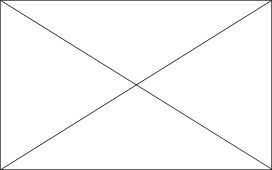
\includegraphics[height=5cm]{Figures/Chapter_1/placeholder} \caption{
			\label{figure_1} One figure using height restriction.}
		\vspace{-0.5cm}
	\end{center}
\end{figure}

\begin{figure}[H] %hbtp
	\begin{center}
		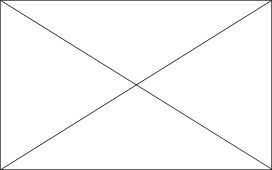
\includegraphics[height=4.5cm]{Figures/Chapter_1/placeholder} 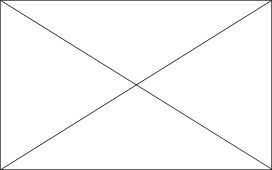
\includegraphics[height=4.5cm]{Figures/Chapter_1/placeholder} \caption{
			\label{figure_2} Two figures using height restriction.}
		\vspace{-0.5cm}
	\end{center}
\end{figure}

\begin{figure}[H] %hbtp
	\begin{center}
		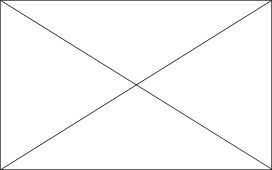
\includegraphics[height=3cm]{Figures/Chapter_1/placeholder} 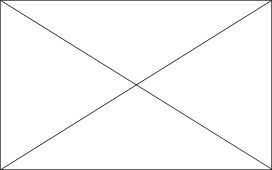
\includegraphics[height=3cm]{Figures/Chapter_1/placeholder} 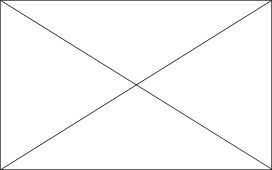
\includegraphics[height=3cm]{Figures/Chapter_1/placeholder} \caption{
			\label{figure_3} Three figures using height restriction.}
		\vspace{-0.5cm}
	\end{center}
\end{figure}

Figures using \textbf{width} restrictions:
\begin{itemize}
	\item One figure (Figure \ref{figure_4})
	\item Two figures (Figure \ref{figure_5})
	\item Three figures (Figure \ref{figure_6})
\end{itemize}

\begin{figure}[H] %hbtp
	\begin{center}
		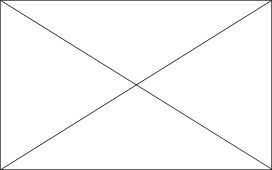
\includegraphics[width=7cm]{Figures/Chapter_1/placeholder} \caption{
			\label{figure_4} One figure using width restriction.}
		\vspace{-0.5cm}
	\end{center}
\end{figure}

\begin{figure}[H] %hbtp
	\begin{center}
		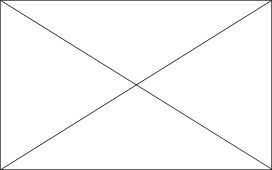
\includegraphics[width=7cm]{Figures/Chapter_1/placeholder} 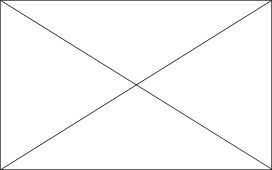
\includegraphics[width=7cm]{Figures/Chapter_1/placeholder} \caption{
			\label{figure_5} Two figures using width restriction.}
		\vspace{-0.5cm}
	\end{center}
\end{figure}

\begin{figure}[H] %hbtp
	\begin{center}
		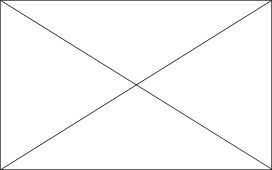
\includegraphics[width=5cm]{Figures/Chapter_1/placeholder} 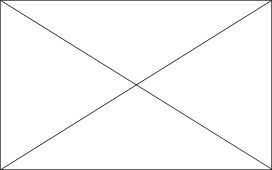
\includegraphics[width=5cm]{Figures/Chapter_1/placeholder} 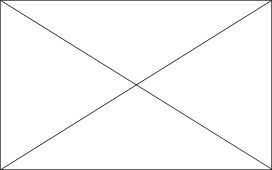
\includegraphics[width=5cm]{Figures/Chapter_1/placeholder} \caption{
			\label{figure_6} Three figures using width restriction.}
		\vspace{-0.5cm}
	\end{center}
\end{figure}

Figures using \textbf{scale} restrictions:
\begin{itemize}
	\item One figure (Figure \ref{figure_7})
	\item Two figures (Figure \ref{figure_8})
	\item Three figures (Figure \ref{figure_9})
\end{itemize}

\begin{figure}[H] %hbtp
	\begin{center}
		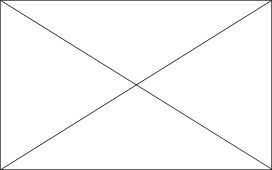
\includegraphics[keepaspectratio=true, scale = 0.75]{Figures/Chapter_1/placeholder} \caption{
			\label{figure_7} One figure using scale restriction.}
		\vspace{-0.5cm}
	\end{center}
\end{figure}

\begin{figure}[H] %hbtp
	\begin{center}
		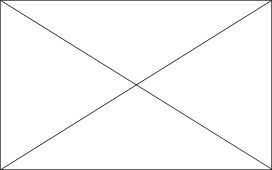
\includegraphics[keepaspectratio=true, scale = 0.6]{Figures/Chapter_1/placeholder} 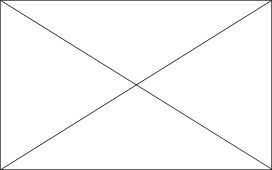
\includegraphics[keepaspectratio=true, scale = 0.6]{Figures/Chapter_1/placeholder} \caption{
			\label{figure_8} Two figures using scale restriction.}
		\vspace{-0.5cm}
	\end{center}
\end{figure}

\begin{figure}[H] %hbtp
	\begin{center}
		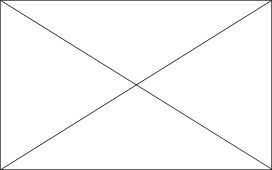
\includegraphics[keepaspectratio=true, scale = 0.5]{Figures/Chapter_1/placeholder} 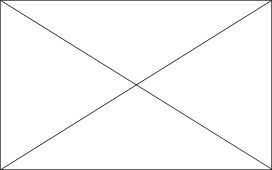
\includegraphics[keepaspectratio=true, scale = 0.5]{Figures/Chapter_1/placeholder} 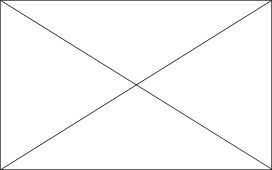
\includegraphics[keepaspectratio=true, scale = 0.5]{Figures/Chapter_1/placeholder} \caption{
			\label{figure_9} Three figures using scale restriction.}
		\vspace{-0.5cm}
	\end{center}
\end{figure}

%% SECTION HEADER /////////////////////////////////////////////////////////////////////////////////////
\section{Example: Equations}
\label{sec12}

%% SECTION CONTENT ////////////////////////////////////////////////////////////////////////////////////

This section shows a few equation examples. Labels can be used to reference equations.
\begin{itemize}
	\item Example (Equation \ref{eq:1_1})
	\item Example (Equation \ref{eq:1_2})
	\item Example (Equation \ref{eq:1_3})
	\item Example (Equation \ref{eq:1_4})
	\item Example (Equation \ref{eq:1_5})
\end{itemize}

\begin{equation}
\label{eq:1_1}
\overline{M}_{i}=\iint\limits_A \rho\;u_{i}\left(u_{k}\;n_{k} \right)\;dA
\end{equation}

\begin{equation}
\label{eq:1_2}
V_{REF} = \left( \frac{2 \times 144 \times P_{DYN}}{\rho} \right)^{\frac{1}{2}}
\end{equation}

\begin{equation}
\label{eq:1_3}
V_{MOM} = \left( \frac{A_{TIP} (\frac{V_{REF}}{2})^{2} + A_{MIDDLE} V_{REF}^{2} + A_{HUB} V_{HUB}^{2}}{A_{JET} V_{AVG}} \right)
\end{equation}

\begin{equation}
\label{eq:1_4}
\begin{aligned}
& Q_{J}= \int_0^\delta Vdy+\left(y-\delta \right)b\;V_{s}\\
& Q_{J}= b\;V_{s} \int_0^\delta \left(\frac{y}{\delta} \right)^\frac{1}{n}dy+\left(y-\delta \right)b\;V_{s}\\
& Q_{J}=\frac{b\;V_{s}}{\left(\frac{n+1}{n} \right)}\delta+\left(y-\delta \right)b\;V_{s}\\
& Q_{J}=b\;V_{s}\left(y-\frac{\delta}{n+1} \right)
\end{aligned}
\end{equation}

\begin{equation}
\label{eq:1_5}
B_{K_{T_{Jx}}}=\sqrt{\left(\theta_{Q_{J}}B_{Q_{J}} \right )^{2}+\left(\theta_{D}B_{D} \right )^{2}+\left(\theta_{n}B_{n} \right )^{2}+\left(\theta_{ \alpha }B_{ \alpha } \right )^{2}+\left(\theta_{\rho}\left(B_{\rho}+\theta_{\rho tw}B_{tw} \right ) \right )}
\end{equation}

%% SECTION HEADER /////////////////////////////////////////////////////////////////////////////////////
\section{Example: Tables}
\label{sec13}

%% SECTION CONTENT ////////////////////////////////////////////////////////////////////////////////////

This section shows a few table examples. Labels can be used to reference tables.
\begin{itemize}
	\item Example (Table \ref{table_1})
	\item Example (Table \ref{table_2})
	\item Example (Table \ref{table_3})	
\end{itemize}

\begin{table}[hbtp]
	\centering
	\caption{Example table for principal ship particulars.}
	\label{table_1}		
	\begin{tabular}{r|c|c|c}
		\toprule
		\multicolumn{4}{c}{\textbf{General particulars}} \\
		\midrule 
		\textbf{Parameter} & \textbf{Acronym} & \textbf{Unit} & \textbf{Value} \\ 
		\midrule 
		Length overall 		& L\textsubscript{OA}   		& m     & 97.2 \\
		Length waterline 	& L\textsubscript{WL}   		& m     & 92.0 \\
		Beam overall 		& B\textsubscript{OA}   		& m     & 26.6 \\
		Beam of demihull 	& B\textsubscript{OA, demihull} & m     & 4.5 \\
		Demihull distance 	& C\textsubscript{L, demihull} 	& m     & 22.1 \\
		Loaded draft 		& T\textsubscript{Loaded} 		& m     & 3.43 \\
		\midrule 	    
		\multicolumn{4}{c}{\textbf{Speed}} \\
		\midrule 
		\textbf{Parameter} & \textbf{Acronym} & \textbf{Unit} & \textbf{Value} \\
		\midrule 	
		Speed at 600t deadweight 	& V\textsubscript{600t}	 & knots 	& 38 \\
		Speed at 300t deadweight	& V\textsubscript{300t}  & knots   	& 42 \\
		\bottomrule
	\end{tabular}
\end{table}

\begin{table}[H] %hbtp
	\centering
	\caption{Example table for summarized data.}
	\label{table_2}		
	\begin{tabular}{c|c|c|c|c|c|c|c|c|c|c}
		\toprule 
		$\boldsymbol{L_{OA}}$ & $\boldsymbol{L_{WL}}$ & $\boldsymbol{B_{OA}}$ & $\boldsymbol{B_{DH}}$ & $\boldsymbol{T}$ & $\boldsymbol{\lambda}$ & $\boldsymbol{B_{DH>200mm}}$  & $\boldsymbol{F_{r@28knots}}$ & $\boldsymbol{\frac{A_{C}}{A_{M}}}$ & $\boldsymbol{\frac{h}{T}}$ & $\boldsymbol{\frac{W}{B}}$ \\
		\cmidrule(lr{.75em}){1-11}  
		m & m & m & m & m & - & - & - & - & - & - \\
		\midrule 
		3.0 & 2.84 & 0.82 & 0.14 & 0.11 & 32.4 & No  & $<$ 0.8 & 362 & 14 & 26 \\
		3.3 & 3.12 & 0.90 & 0.15 & 0.12 & 29.5 & No  & $<$ 0.8 & 299 & 13 & 23 \\
		3.6 & 3.41 & 0.98 & 0.17 & 0.13 & 27.0 & No  & $<$ 0.8 & 252 & 12 & 21 \\
		\bottomrule
	\end{tabular}
\end{table}

\begin{table}[H] %hbtp
	\centering
	\caption{Example table showing merged cells.}
	\label{table_3}		
	\begin{tabular}{c|c|c|c|c|c|c}
		\toprule
		\textbf{F\textsubscript{r}} & $\boldsymbol{\theta_{S}B_{S}}$ & $\boldsymbol{\theta_{V}B_{V}}$ & $\boldsymbol{\theta_{Mx}B_{Mx}}$ & $\boldsymbol{\theta_{\rho}(B_{\rho}+\theta_{\rho tw}B_{tw})}$ & \textbf{B\textsubscript{CT}} & \textbf{P\textsubscript{CT}} \\
		\cmidrule(lr{.75em}){1-7}
		- & - & - & - & - & - & - \\
		\midrule
		\multicolumn{7}{c}{\textbf{Condition 1}} \\
		\midrule
		0.23  & -3.40E-05 & -3.26E-06 & 1.23E-04 & -6.28E-06 & 1.28E-04 & 1.30E-05 \\
		0.26  & -3.67E-05 & -3.09E-06 & 9.49E-05 & -6.77E-06 & 1.02E-04 & 4.45E-05 \\
		0.28  & -3.65E-05 & -2.86E-06 & 8.22E-05 & -6.74E-06 & 9.03E-05 & 1.30E-05 \\
		0.29  & -3.68E-05 & -2.80E-06 & 7.72E-05 & -6.80E-06 & 8.58E-05 & 2.83E-05 \\
		0.31  & -3.75E-05 & -2.66E-06 & 6.75E-05 & -6.92E-06 & 7.76E-05 & 4.50E-05 \\
		\midrule
		\multicolumn{7}{c}{\textbf{Condition 2}} \\
		\midrule
		0.23  & -3.23E-05 & -3.10E-06 & 1.25E-04 & -5.97E-06 & 1.29E-04 & 2.52E-05 \\
		0.29  & -3.38E-05 & -2.57E-06 & 7.82E-05 & -6.24E-06 & 8.54E-05 & 7.14E-06 \\
		0.35  & -3.10E-05 & -1.95E-06 & 5.35E-05 & -5.73E-06 & 6.21E-05 & 1.66E-05 \\
		0.41  & -3.30E-05 & -1.76E-06 & 3.89E-05 & -6.08E-06 & 5.13E-05 & 3.71E-05 \\
		0.47  & -3.33E-05 & -1.56E-06 & 2.96E-05 & -6.15E-06 & 4.50E-05 & 1.05E-05 \\
		\midrule
		\multicolumn{7}{c}{\textbf{Condition 3}} \\
		\midrule
		0.23  & -3.50E-05 & -3.36E-06 & 1.22E-04 & -6.46E-06 & 1.27E-04 & 1.25E-05 \\
		0.29  & -3.83E-05 & -2.90E-06 & 7.60E-05 & -7.06E-06 & 8.54E-05 & 1.45E-05 \\
		0.35  & -3.68E-05 & -2.31E-06 & 5.19E-05 & -6.79E-06 & 6.40E-05 & 8.99E-06 \\
		0.42  & -3.70E-05 & -1.98E-06 & 3.78E-05 & -6.82E-06 & 5.33E-05 & 2.65E-05 \\
		0.48  & -3.53E-05 & -1.65E-06 & 2.87E-05 & -6.52E-06 & 4.60E-05 & 5.67E-06 \\
		\bottomrule
	\end{tabular}
\end{table}

%% SECTION HEADER /////////////////////////////////////////////////////////////////////////////////////
\section{Example: Referencing}
\label{sec14}

%% SECTION CONTENT ////////////////////////////////////////////////////////////////////////////////////

This section shows a few referencing examples. The reference system used is ''BibTex'' and the BibTex file is located in ''/References/thesis.bib''. The LaTeX reference package for styling references/bibliography is ''BibLaTex'' and in-text references can be added by using ''\textcite{}'' as shown in the following examples:
\begin{itemize}
	\item Example \textbf{article} reference: \textcite{Allison2001}
	\item Example \textbf{book} reference: \textcite{Bose2008}
	\item Example \textbf{conference paper} reference: \textcite{Chakrabarti1998}
	\item Example \textbf{proceedings} reference: \textcite{Jessup2008}
	\item Example \textbf{thesis} reference: \textcite{BultenPhD2006}
	\item Example \textbf{report} reference: \textcite{Bowden1974}		
\end{itemize}
For styling of references/bibliography see line 160 in ''/Packages/mathphdthesis.sty''. Configuration settings for ''BibLaTeX'' can be found here:
\begin{itemize}
	\item \href{http://ctan.unsw.edu.au/macros/latex/contrib/biblatex/doc/biblatex.pdf}{http://ctan.unsw.edu.au/macros/latex/contrib/biblatex/doc/biblatex.pdf}
	\item \href{http://tex.stackexchange.com/questions/13509/biblatex-for-idiots}{http://tex.stackexchange.com/questions/13509/biblatex-for-idiots}
	\item \href{https://www.sharelatex.com/blog/2013/07/31/getting-started-with-biblatex.html}{https://www.sharelatex.com/blog/2013/07/31/getting-started-with-biblatex.html}
\end{itemize}


% Note that the text in the [] brackets is the one that will
% appear in the table of contents, whilst the text in the {}
% brackets will appear in the main thesis.

%% CHAPTER HEADER /////////////////////////////////////////////////////////////////////////////////////
\chapter[Section 2]{Section 2}
\label{ch2}

%% CHAPTER INTRODUCTION ///////////////////////////////////////////////////////////////////////////////

\lipsum[1]

%% INCLUDE SECTIONS ///////////////////////////////////////////////////////////////////////////////////

%% SECTION HEADER /////////////////////////////////////////////////////////////////////////////////////
\section{Subsection}
\label{sec21}

%% SECTION CONTENT ////////////////////////////////////////////////////////////////////////////////////

\lipsum[1]

%% SUBSECTION HEADER //////////////////////////////////////////////////////////////////////////////////
\subsection{Subsubsection}
\label{sec211}

\lipsum[1]

%% SUBSECTION HEADER //////////////////////////////////////////////////////////////////////////////////
\subsection{Subsubsection}
\label{sec212}

\lipsum[1]

%% SUBSECTION HEADER //////////////////////////////////////////////////////////////////////////////////
\subsection{Subsubsection}
\label{sec213}

\lipsum[1]

%% SECTION HEADER /////////////////////////////////////////////////////////////////////////////////////
\section{Subsection}
\label{sec22}

%% SECTION CONTENT ////////////////////////////////////////////////////////////////////////////////////

\lipsum[1]

%% SUBSECTION HEADER //////////////////////////////////////////////////////////////////////////////////
\subsection{Subsubsection}
\label{sec221}

\lipsum[1]

%% SUBSECTION HEADER //////////////////////////////////////////////////////////////////////////////////
\subsection{Subsubsection}
\label{sec222}

\lipsum[1]

%% SUBSECTION HEADER //////////////////////////////////////////////////////////////////////////////////
\subsection{Subsubsection}
\label{sec223}

\lipsum[1]

%% SECTION HEADER /////////////////////////////////////////////////////////////////////////////////////
\section{Subsection}
\label{sec23}

%% SECTION CONTENT ////////////////////////////////////////////////////////////////////////////////////

\lipsum[1]

%% SUBSECTION HEADER //////////////////////////////////////////////////////////////////////////////////
\subsection{Subsubsection}
\label{sec231}

\lipsum[1]

%% SUBSECTION HEADER //////////////////////////////////////////////////////////////////////////////////
\subsection{Subsubsection}
\label{sec232}

\lipsum[1]

%% SUBSECTION HEADER //////////////////////////////////////////////////////////////////////////////////
\subsection{Subsubsection}
\label{sec233}

\lipsum[1]


% Note that the text in the [] brackets is the one that will
% appear in the table of contents, whilst the text in the {}
% brackets will appear in the main thesis.

%% CHAPTER HEADER /////////////////////////////////////////////////////////////////////////////////////
\chapter[Section 3]{Section 3}
\label{ch3}

%% CHAPTER INTRODUCTION ///////////////////////////////////////////////////////////////////////////////

\lipsum[1]

%% INCLUDE SECTIONS ///////////////////////////////////////////////////////////////////////////////////

%% SECTION HEADER /////////////////////////////////////////////////////////////////////////////////////
\section{Subsection}
\label{sec31}

%% SECTION CONTENT ////////////////////////////////////////////////////////////////////////////////////

\lipsum[1]

%% SUBSECTION HEADER //////////////////////////////////////////////////////////////////////////////////
\subsection{Subsubsection}
\label{sec311}

\lipsum[1]

%% SUBSECTION HEADER //////////////////////////////////////////////////////////////////////////////////
\subsection{Subsubsection}
\label{sec312}

\lipsum[1]

%% SUBSECTION HEADER //////////////////////////////////////////////////////////////////////////////////
\subsection{Subsubsection}
\label{sec313}

\lipsum[1]

%% SECTION HEADER /////////////////////////////////////////////////////////////////////////////////////
\section{Subsection}
\label{sec32}

%% SECTION CONTENT ////////////////////////////////////////////////////////////////////////////////////

\lipsum[1]

%% SUBSECTION HEADER //////////////////////////////////////////////////////////////////////////////////
\subsection{Subsubsection}
\label{sec321}

\lipsum[1]

%% SUBSECTION HEADER //////////////////////////////////////////////////////////////////////////////////
\subsection{Subsubsection}
\label{sec322}

\lipsum[1]

%% SUBSECTION HEADER //////////////////////////////////////////////////////////////////////////////////
\subsection{Subsubsection}
\label{sec323}

\lipsum[1]

%% SECTION HEADER /////////////////////////////////////////////////////////////////////////////////////
\section{Subsection}
\label{sec33}

%% SECTION CONTENT ////////////////////////////////////////////////////////////////////////////////////

\lipsum[1]

%% SUBSECTION HEADER //////////////////////////////////////////////////////////////////////////////////
\subsection{Subsubsection}
\label{sec331}

\lipsum[1]

%% SUBSECTION HEADER //////////////////////////////////////////////////////////////////////////////////
\subsection{Subsubsection}
\label{sec332}

\lipsum[1]

%% SUBSECTION HEADER //////////////////////////////////////////////////////////////////////////////////
\subsection{Subsubsection}
\label{sec333}

\lipsum[1]


% Note that the text in the [] brackets is the one that will
% appear in the table of contents, whilst the text in the {}
% brackets will appear in the main thesis.

%% CHAPTER HEADER /////////////////////////////////////////////////////////////////////////////////////
\chapter[Section 4]{Section 4}
\label{ch4}

%% CHAPTER INTRODUCTION ///////////////////////////////////////////////////////////////////////////////

\lipsum[1]

%% INCLUDE SECTIONS ///////////////////////////////////////////////////////////////////////////////////

%% SECTION HEADER /////////////////////////////////////////////////////////////////////////////////////
\section{Subsection}
\label{sec41}

%% SECTION CONTENT ////////////////////////////////////////////////////////////////////////////////////

\lipsum[1]

%% SUBSECTION HEADER //////////////////////////////////////////////////////////////////////////////////
\subsection{Subsubsection}
\label{sec411}

\lipsum[1]

%% SUBSECTION HEADER //////////////////////////////////////////////////////////////////////////////////
\subsection{Subsubsection}
\label{sec412}

\lipsum[1]

%% SUBSECTION HEADER //////////////////////////////////////////////////////////////////////////////////
\subsection{Subsubsection}
\label{sec413}

\lipsum[1]

%% SECTION HEADER /////////////////////////////////////////////////////////////////////////////////////
\section{Subsection}
\label{sec42}

%% SECTION CONTENT ////////////////////////////////////////////////////////////////////////////////////

\lipsum[1]

%% SUBSECTION HEADER //////////////////////////////////////////////////////////////////////////////////
\subsection{Subsubsection}
\label{sec421}

\lipsum[1]

%% SUBSECTION HEADER //////////////////////////////////////////////////////////////////////////////////
\subsection{Subsubsection}
\label{sec422}

\lipsum[1]

%% SUBSECTION HEADER //////////////////////////////////////////////////////////////////////////////////
\subsection{Subsubsection}
\label{sec423}

\lipsum[1]

%% SECTION HEADER /////////////////////////////////////////////////////////////////////////////////////
\section{Subsection}
\label{sec43}

%% SECTION CONTENT ////////////////////////////////////////////////////////////////////////////////////

\lipsum[1]

%% SUBSECTION HEADER //////////////////////////////////////////////////////////////////////////////////
\subsection{Subsubsection}
\label{sec431}

\lipsum[1]

%% SUBSECTION HEADER //////////////////////////////////////////////////////////////////////////////////
\subsection{Subsubsection}
\label{sec432}

\lipsum[1]

%% SUBSECTION HEADER //////////////////////////////////////////////////////////////////////////////////
\subsection{Subsubsection}
\label{sec433}

\lipsum[1]


% Note that the text in the [] brackets is the one that will
% appear in the table of contents, whilst the text in the {}
% brackets will appear in the main thesis.

%% CHAPTER HEADER /////////////////////////////////////////////////////////////////////////////////////
\chapter[Section 5]{Section 5}
\label{ch5}

%% CHAPTER INTRODUCTION ///////////////////////////////////////////////////////////////////////////////

\lipsum[1]

%% INCLUDE SECTIONS ///////////////////////////////////////////////////////////////////////////////////

%% SECTION HEADER /////////////////////////////////////////////////////////////////////////////////////
\section{Subsection}
\label{sec51}

%% SECTION CONTENT ////////////////////////////////////////////////////////////////////////////////////

\lipsum[1]

%% SUBSECTION HEADER //////////////////////////////////////////////////////////////////////////////////
\subsection{Subsubsection}
\label{sec511}

\lipsum[1]

%% SUBSECTION HEADER //////////////////////////////////////////////////////////////////////////////////
\subsection{Subsubsection}
\label{sec512}

\lipsum[1]

%% SUBSECTION HEADER //////////////////////////////////////////////////////////////////////////////////
\subsection{Subsubsection}
\label{sec513}

\lipsum[1]

%% SECTION HEADER /////////////////////////////////////////////////////////////////////////////////////
\section{Subsection}
\label{sec52}

%% SECTION CONTENT ////////////////////////////////////////////////////////////////////////////////////

\lipsum[1]

%% SUBSECTION HEADER //////////////////////////////////////////////////////////////////////////////////
\subsection{Subsubsection}
\label{sec521}

\lipsum[1]

%% SUBSECTION HEADER //////////////////////////////////////////////////////////////////////////////////
\subsection{Subsubsection}
\label{sec522}

\lipsum[1]

%% SUBSECTION HEADER //////////////////////////////////////////////////////////////////////////////////
\subsection{Subsubsection}
\label{sec523}

\lipsum[1]

%% SECTION HEADER /////////////////////////////////////////////////////////////////////////////////////
\section{Subsection}
\label{sec53}

%% SECTION CONTENT ////////////////////////////////////////////////////////////////////////////////////

\lipsum[1]

%% SUBSECTION HEADER //////////////////////////////////////////////////////////////////////////////////
\subsection{Subsubsection}
\label{sec531}

\lipsum[1]

%% SUBSECTION HEADER //////////////////////////////////////////////////////////////////////////////////
\subsection{Subsubsection}
\label{sec532}

\lipsum[1]

%% SUBSECTION HEADER //////////////////////////////////////////////////////////////////////////////////
\subsection{Subsubsection}
\label{sec533}

\lipsum[1]


% Note that the text in the [] brackets is the one that will
% appear in the table of contents, whilst the text in the {}
% brackets will appear in the main thesis.

%% CHAPTER HEADER /////////////////////////////////////////////////////////////////////////////////////
\chapter[Section 6]{Section 7}
\label{ch6}

%% CHAPTER INTRODUCTION ///////////////////////////////////////////////////////////////////////////////

\lipsum[1]

%% INCLUDE SECTIONS ///////////////////////////////////////////////////////////////////////////////////

%% SECTION HEADER /////////////////////////////////////////////////////////////////////////////////////
\section{Subsection}
\label{sec61}

%% SECTION CONTENT ////////////////////////////////////////////////////////////////////////////////////

\lipsum[1]

%% SUBSECTION HEADER //////////////////////////////////////////////////////////////////////////////////
\subsection{Subsubsection}
\label{sec611}

\lipsum[1]

%% SUBSECTION HEADER //////////////////////////////////////////////////////////////////////////////////
\subsection{Subsubsection}
\label{sec612}

\lipsum[1]

%% SUBSECTION HEADER //////////////////////////////////////////////////////////////////////////////////
\subsection{Subsubsection}
\label{sec613}

\lipsum[1]

%% SECTION HEADER /////////////////////////////////////////////////////////////////////////////////////
\section{Subsection}
\label{sec62}

%% SECTION CONTENT ////////////////////////////////////////////////////////////////////////////////////

\lipsum[1]

%% SUBSECTION HEADER //////////////////////////////////////////////////////////////////////////////////
\subsection{Subsubsection}
\label{sec621}

\lipsum[1]

%% SUBSECTION HEADER //////////////////////////////////////////////////////////////////////////////////
\subsection{Subsubsection}
\label{sec622}

\lipsum[1]

%% SUBSECTION HEADER //////////////////////////////////////////////////////////////////////////////////
\subsection{Subsubsection}
\label{sec623}

\lipsum[1]

%% SECTION HEADER /////////////////////////////////////////////////////////////////////////////////////
\section{Subsection}
\label{sec63}

%% SECTION CONTENT ////////////////////////////////////////////////////////////////////////////////////

\lipsum[1]

%% SUBSECTION HEADER //////////////////////////////////////////////////////////////////////////////////
\subsection{Subsubsection}
\label{sec631}

\lipsum[1]

%% SUBSECTION HEADER //////////////////////////////////////////////////////////////////////////////////
\subsection{Subsubsection}
\label{sec632}

\lipsum[1]

%% SUBSECTION HEADER //////////////////////////////////////////////////////////////////////////////////
\subsection{Subsubsection}
\label{sec633}

\lipsum[1]


% Note that the text in the [] brackets is the one that will
% appear in the table of contents, whilst the text in the {}
% brackets will appear in the main thesis.

%% CHAPTER HEADER /////////////////////////////////////////////////////////////////////////////////////
\chapter[Section 7]{Section 7}
\label{ch7}

%% CHAPTER INTRODUCTION ///////////////////////////////////////////////////////////////////////////////

\lipsum[1]

%% INCLUDE SECTIONS ///////////////////////////////////////////////////////////////////////////////////

%% SECTION HEADER /////////////////////////////////////////////////////////////////////////////////////
\section{Subsection}
\label{sec71}

%% SECTION CONTENT ////////////////////////////////////////////////////////////////////////////////////

\lipsum[1]

%% SUBSECTION HEADER //////////////////////////////////////////////////////////////////////////////////
\subsection{Subsubsection}
\label{sec711}

\lipsum[1]

%% SUBSECTION HEADER //////////////////////////////////////////////////////////////////////////////////
\subsection{Subsubsection}
\label{sec712}

\lipsum[1]

%% SUBSECTION HEADER //////////////////////////////////////////////////////////////////////////////////
\subsection{Subsubsection}
\label{sec713}

\lipsum[1]

%% SECTION HEADER /////////////////////////////////////////////////////////////////////////////////////
\section{Subsection}
\label{sec72}

%% SECTION CONTENT ////////////////////////////////////////////////////////////////////////////////////

\lipsum[1]

%% SUBSECTION HEADER //////////////////////////////////////////////////////////////////////////////////
\subsection{Subsubsection}
\label{sec721}

\lipsum[1]

%% SUBSECTION HEADER //////////////////////////////////////////////////////////////////////////////////
\subsection{Subsubsection}
\label{sec722}

\lipsum[1]

%% SUBSECTION HEADER //////////////////////////////////////////////////////////////////////////////////
\subsection{Subsubsection}
\label{sec723}

\lipsum[1]

%% SECTION HEADER /////////////////////////////////////////////////////////////////////////////////////
\section{Subsection}
\label{sec73}

%% SECTION CONTENT ////////////////////////////////////////////////////////////////////////////////////

\lipsum[1]

%% SUBSECTION HEADER //////////////////////////////////////////////////////////////////////////////////
\subsection{Subsubsection}
\label{sec731}

\lipsum[1]

%% SUBSECTION HEADER //////////////////////////////////////////////////////////////////////////////////
\subsection{Subsubsection}
\label{sec732}

\lipsum[1]

%% SUBSECTION HEADER //////////////////////////////////////////////////////////////////////////////////
\subsection{Subsubsection}
\label{sec733}

\lipsum[1]


% app0.tex (file to switch to appendix mode)
% No need to alter this file...
\appendix

% Note that the text in the [] brackets is the one that will
% appear in the table of contents, whilst the text in the {}
% brackets will appear in the main thesis.

%% APPENDIX HEADER ////////////////////////////////////////////////////////////////////////////////////
\chapter[Appendix 1]{Appendix 1}
\label{appa}

%% APPENDIX CONTENT ///////////////////////////////////////////////////////////////////////////////////

\lipsum[1]

% Note that the text in the [] brackets is the one that will
% appear in the table of contents, whilst the text in the {}
% brackets will appear in the main thesis.

%% APPENDIX HEADER ////////////////////////////////////////////////////////////////////////////////////
\chapter[Appendix 2]{Appendix 2}
\label{appb}

%% APPENDIX CONTENT ///////////////////////////////////////////////////////////////////////////////////

\lipsum[1]

% Note that the text in the [] brackets is the one that will
% appear in the table of contents, whilst the text in the {}
% brackets will appear in the main thesis.

%% APPENDIX HEADER ////////////////////////////////////////////////////////////////////////////////////
\chapter[Appendix 3]{Appendix 3}
\label{appc}

%% APPENDIX CONTENT ///////////////////////////////////////////////////////////////////////////////////

\lipsum[1]

% Note that the text in the [] brackets is the one that will
% appear in the table of contents, whilst the text in the {}
% brackets will appear in the main thesis.

%% APPENDIX HEADER ////////////////////////////////////////////////////////////////////////////////////
\chapter[Appendix 4]{Appendix 4}
\label{appd}

%% APPENDIX CONTENT ///////////////////////////////////////////////////////////////////////////////////

\lipsum[1]

% Note that the text in the [] brackets is the one that will
% appear in the table of contents, whilst the text in the {}
% brackets will appear in the main thesis.

%% APPENDIX HEADER ////////////////////////////////////////////////////////////////////////////////////
\chapter[Appendix 5]{Appendix 5}
\label{appe}

%% APPENDIX CONTENT ///////////////////////////////////////////////////////////////////////////////////

\lipsum[1]

% Note that the text in the [] brackets is the one that will
% appear in the table of contents, whilst the text in the {}
% brackets will appear in the main thesis.

%% APPENDIX HEADER ////////////////////////////////////////////////////////////////////////////////////
\chapter[Appendix 6]{Appendix 6}
\label{appf}

%% APPENDIX CONTENT ///////////////////////////////////////////////////////////////////////////////////

\lipsum[1]

% Note that the text in the [] brackets is the one that will
% appear in the table of contents, whilst the text in the {}
% brackets will appear in the main thesis.

%% APPENDIX HEADER ////////////////////////////////////////////////////////////////////////////////////
\chapter[Appendix 7]{Appendix 7}
\label{appg}

%% APPENDIX CONTENT ///////////////////////////////////////////////////////////////////////////////////

\lipsum[1]

% A small file that prints the index in the main document.
% No need to alter this file...
\printindex


% Bibliography
\addcontentsline{toc}{chapter}{References/Bibliography}
\printbibliography

\end{document}
